%%%%%%%%%%%%%%%% NÃO ALTERE O CAMPO ABAIXO 
\documentclass[10pt,twoside,a4paper]{article}
\usepackage[T1]{fontenc}
\usepackage[utf8]{inputenc}
\usepackage[portuges]{babel}
\usepackage[a4paper]{geometry}
\geometry{tmargin=1.2cm,bmargin=1.7cm,lmargin=1.5cm,rmargin=1.5cm}
\usepackage{graphicx}
\usepackage{indentfirst}
\usepackage{subcaption} % figuras lado a lado
\usepackage{booktabs} %tabelas
\usepackage{url}% web links
\usepackage{semat}
\usepackage{lipsum} %Texto automático
\usepackage{amsthm, amsmath, amssymb, wasysym, MnSymbol}
%%%%%%%%%%%%%%%%

%%%%%%%%%%%%%%%% Se necessitar de pacotes adicionais insira abaixo
\usepackage{verbatim}
%%%%%%%%%%%%%%%%%%%%%%%%%%%%%%%%

%%%%%%%%%%%%%%%%%%
% Evite redefinir ou criar comandos, por exemplo:
% \R=\mathbb{R} ,\newtheorem{teo}{Teorema}, etc
% Isto pode gerar conflito quando os trabalhos forem
% compilados juntos para o caderno de resumos
\newtheorem{theorem}{Teorema}
\newtheorem{proposition}[theorem]{Proposição}
\newtheorem{lemma}[theorem]{Lema}
\newtheorem{definition}[theorem]{Definição}
\newtheorem{corollary}[theorem]{Corolário}
\renewcommand{\qedsymbol}{$\blacksquare$}
\renewcommand{\sin}{{\rm{sen}\hspace{2pt}}}
\renewcommand{\sinh}{{\rm{senh}\hspace{2pt}}}
%%%%%%%%%%%%%%

%%%%%%%%%%% Não altere os comandos abaixo
\newcommand*{\affaddr}[1]{#1} 
\newcommand*{\affmark}[1][*]{\textsuperscript{#1}}
\newcommand*{\email}[1]{\texttt{#1}}
\usepackage{helvet}% Fonte 
\renewcommand{\familydefault}{\sfdefault}% Fonte 
\renewcommand\Authands{ e }
\evento{XVIII Semat e VIII Semest}
\date{02 a 05 de outubro de 2018}
%%%%%%%%%%%%%%%%
% Dados do trabalho
\title{A STUDY OF THE MEMRISTOR, 
THE FOURTH CIRCUIT ELEMENT }
% Autores: o primeiro será, necessariamente, o apresentador do trabalho
\author[1]{\underline{Lesly Viviane Montúfar Berrios}\thanks{leslymontufar@ufu.br}}
\author[2]{Segundo Autor Orientador\thanks{autor2@unicamp.br}}
\affil[1]{FEELT - Universidade Federal de Uberlândia}
\affil[2]{FAMAT - Universidade Federal de Uberlândia}
%palavras-chave: insira até três palavras
\keywords{Elemento de Circuito. Memristor. }





%Os titulos das seções são apenas exemplos.
%deve-se manter (obrigatoriamente) as seções Resumo e Referências.
%Compilar o arquivo com PDFLatex
%--------------------------------------------------
\begin{document}
\inserirtitulo
\linespread{1.5}% Espaçamento 1.5
%==================================
% RESUMO
%==================================

\section{Resumo}
O presente trabalho traz uma análise do problema simplificado de modelagem das ondas do mar no plano como
motivação para tratar algumas das equações diferenciais parciais (EDPs) estudadas ao longo do PICME (Programa
de Iniciação Científica e Mestrado). Nesse sentido, as principais características de três diferentes regiões do mar
definem três EDPs para se trabalhar com o problema, a saber, a KdV (Korteweg deVries), a equação da onda e a
equação de Burger. %% POR ÚLTIMO

%==================================
% INTRODUÇÃO
%==================================
\section{Introdução} % apague as linhas abaixo e insira aqui a introdução
\lipsum[2-3] % RESULTADOS PRIMEIRO!

Tal resultado pode ser encontrado em \cite{lamport94}.

%==================================
% Primeira Seção
%==================================
\section{Contexto Histórico} % apague as linhas abaixo e insira aqui a primeira seção

O conceito de um resistor com memória existia mesmo antes da publicação de Leon Chua sobre o memristor em 1971. Em 1960, o professor Bernard Widrow, da Universidade de Stanford, desenvolveu um novo elemento de circuito chamado "memistor". Assim, a resistência do memistor foi controlada pela carga. Memistors formaram os componentes básicos da arquitetura de rede neural chamada ADALINE (ADAptive Linear NEuron).

%% A STUDY OF MEMRISTOR
Em 1971, Leon Chua, propôs que deveria haver um quarto elemento de circuito passivo fundamental para estabelecer uma relação matemática entre $q$ e $\varphi$, que ele chamou de memristor (um portmanteau de memória e resistor) [Chua, 1971]. Chua previu que uma classe de memristores poderia ser realizada na forma de um dispositivo puro de estado sólido sem uma fonte de alimentação interna.

Em 2008, Williams e outros, da Hewlett Packard, anunciaram o primeiro dispositivo memristor fabricado [Strukov et al., 2008]. No entanto, um resistor com memória não é uma coisa nova. Se tomar o exemplo da memória não volátil, ela remonta a 1960, quando Bernard Widrow introduziu um novo elemento de circuito chamado memistor [Widrow et al., 1960]. O motivo para escolher o nome de memistor é exatamente o mesmo que o memristor, um resistor com memória. O memistor possui três terminais e sua resistência é controlada pela integral de tempo de um sinal de corrente de controle. Isso significa que a resistência do memistor é controlada pela carga. Widrow inventou o memistor como um elemento de memória eletrolítica para formar um


\begin{comment}
\begin{theorem}
Este é um exemplo de Teorema
\end{theorem}
\begin{proof}
\lipsum[2]
\end{proof}
\end{comment}

%==================================
% Segunda Seção
%==================================
\section{Definição de um Memristor} % apague as linhas abaixo e insira aqui a segunda seção
\lipsum[5]

Verifique a Figura~\ref{fig:distribuicao}.


\begin{figure}[!ht]
\centering
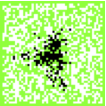
\includegraphics[scale=1.4]{cnmac2}
\caption{Um exemplo de figura.}
\label{fig:distribuicao}
\end{figure}

\lipsum[4]

\begin{proposition}
Este é um exemplo de Proposição
\end{proposition}
\begin{proof}
\lipsum[2]
\end{proof}

\lipsum[3-4]

\begin{figure}[!ht]
\centering
\begin{subfigure}{0.49\textwidth}
\centering
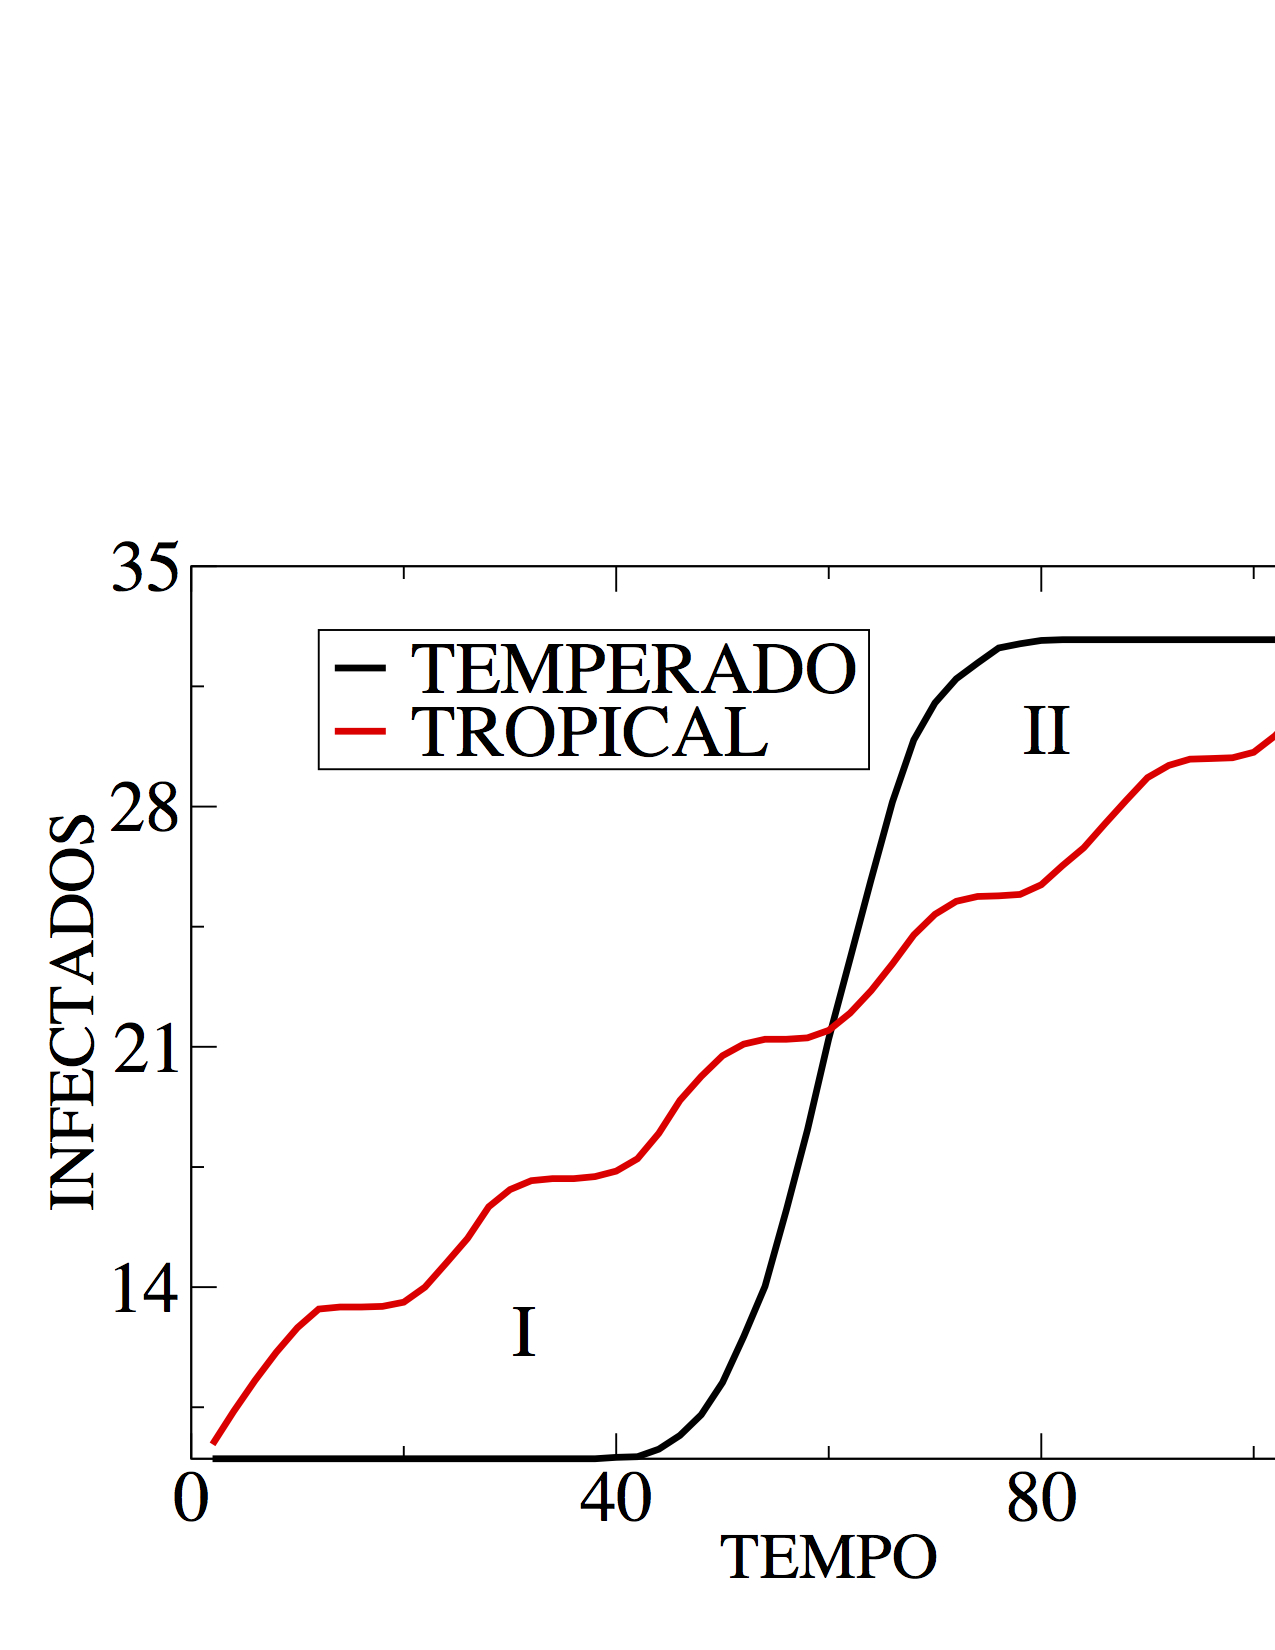
\includegraphics[scale=0.2]{cnmac3}
\caption{Left figure}
\label{fig:left}
\end{subfigure}
\begin{subfigure}{0.49\textwidth}
\centering
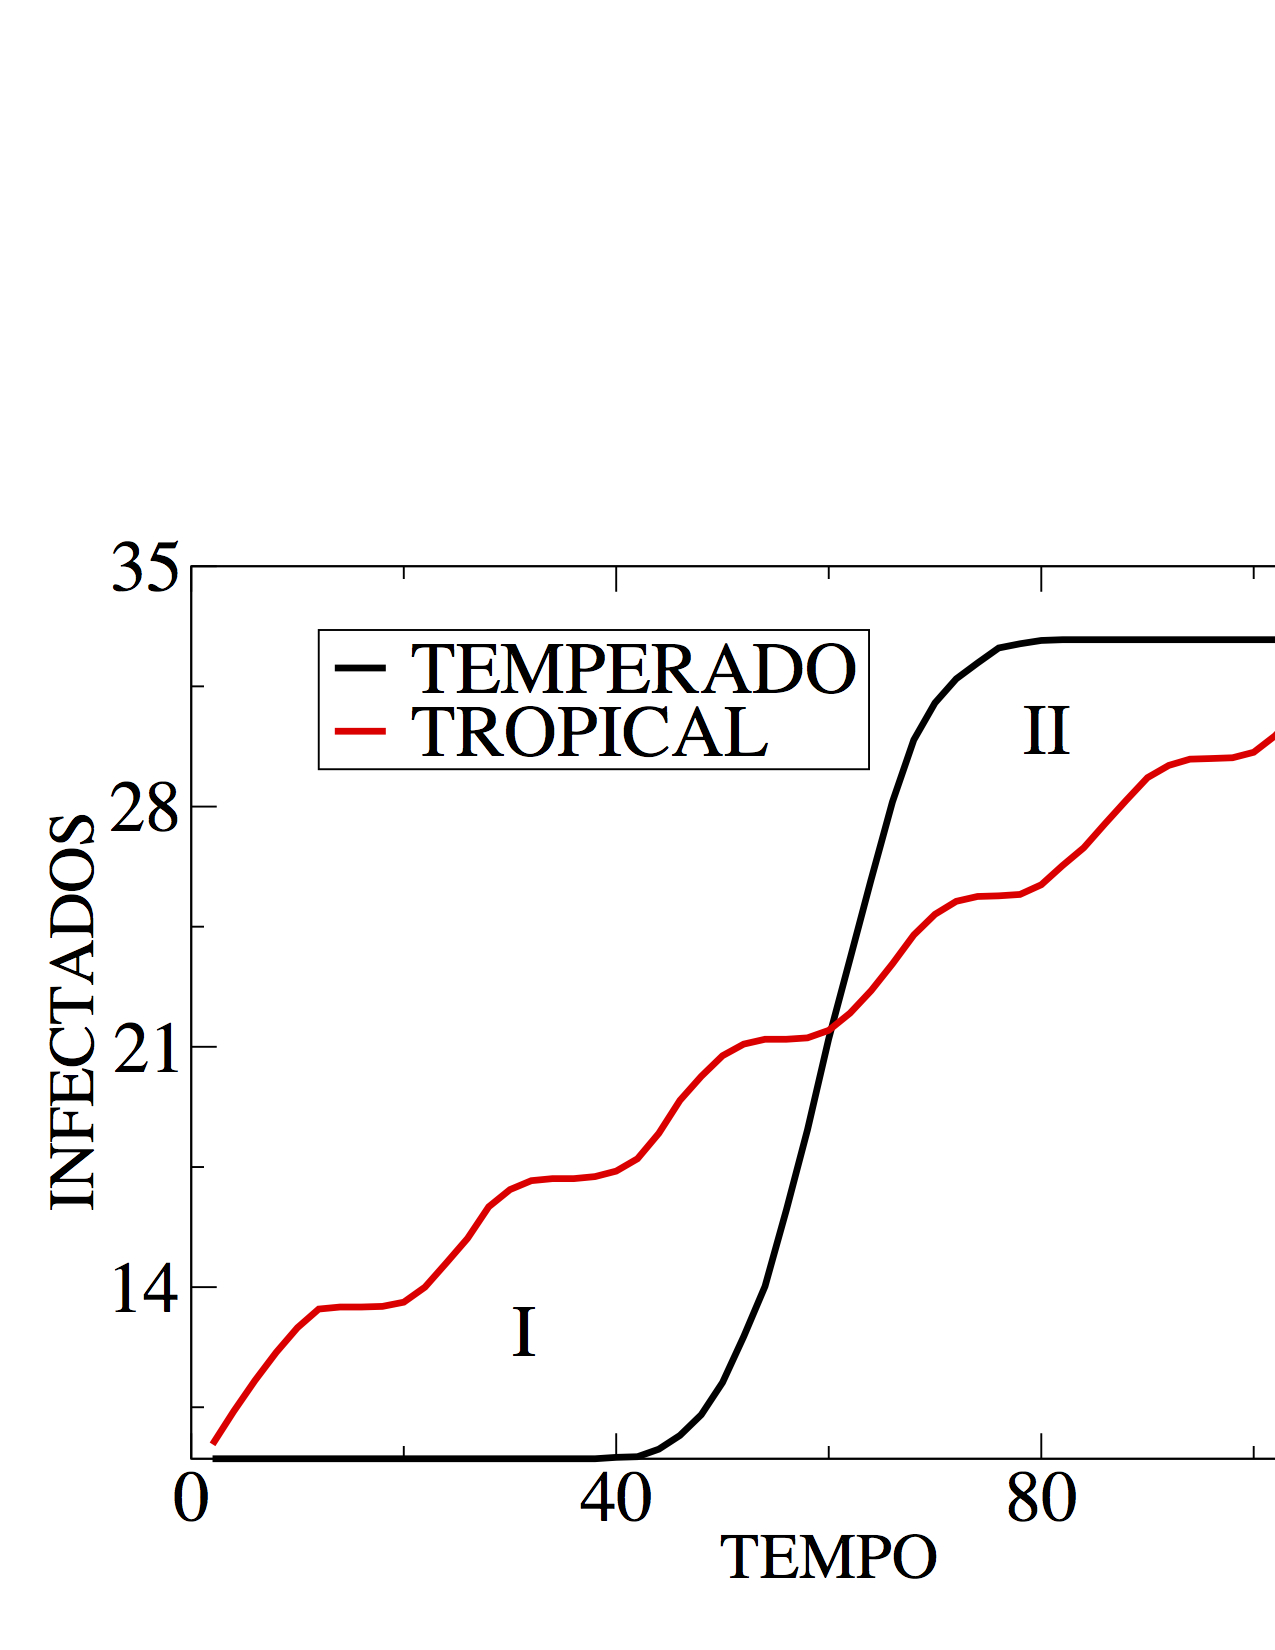
\includegraphics[scale=0.2]{cnmac3}
\caption{Right figure}
\label{fig:right}
\end{subfigure}
\caption{Figuras lado a lado}
\label{fig:combined}
\end{figure}

\lipsum[5]

\begin{center}
Para tabelas, sugerimos a leitura do manual \url{https://www.tug.org/pracjourn/2007-1/mori/mori.pdf}
\end{center}

\begin{table}[h!]
\label{tabela1}
\caption{Maximum  load  and  nominal  tension .}
\centering
\begin{tabular}{clccc}
\toprule
$D$ &               & $P_u$      & $\sigma_N$    \\
(in)&               & (lbs)      & (psi)          \\  \toprule
%
5    & test 1      & 285         & 38.00   \\
& test 2      & 287         & 38.27          \\
& test 3      & 230         & 30.67          \\   \midrule
10   & test 1      & 430         & 28.67   \\
& test 2      & 433         & 28.87          \\
& test 3      & 431         & 28.73          \\    \bottomrule
\end{tabular}
\end{table}



%==================================
% CONCLUSÃO
%==================================
\section{Conclusão} % apague as linhas abaixo e insira aqui a conclusão
\lipsum[8-9]

%==================================
% AGRADECIMENTOS
%==================================
\section{Agradecimentos} % apague as linhas abaixo e insira aqui os agradecimentos
\lipsum[4]


%==================================
% REFERÊNCIAS
%==================================
\begin{thebibliography}{9} % apague as linhas abaixo e insira aqui bibliografia

\bibitem{lamport94}
  Leslie Lamport,
  \emph{\LaTeX: a document preparation system},
  Addison Wesley, Massachusetts,
  2nd edition,
  1994.

\bibitem{pchave2}
  Leslie Lamport,
  \emph{\LaTeX: a document preparation system},
  Addison Wesley, Massachusetts,
  2nd edition,
  1994.

\end{thebibliography}

%--- FIM ---
\end{document}
